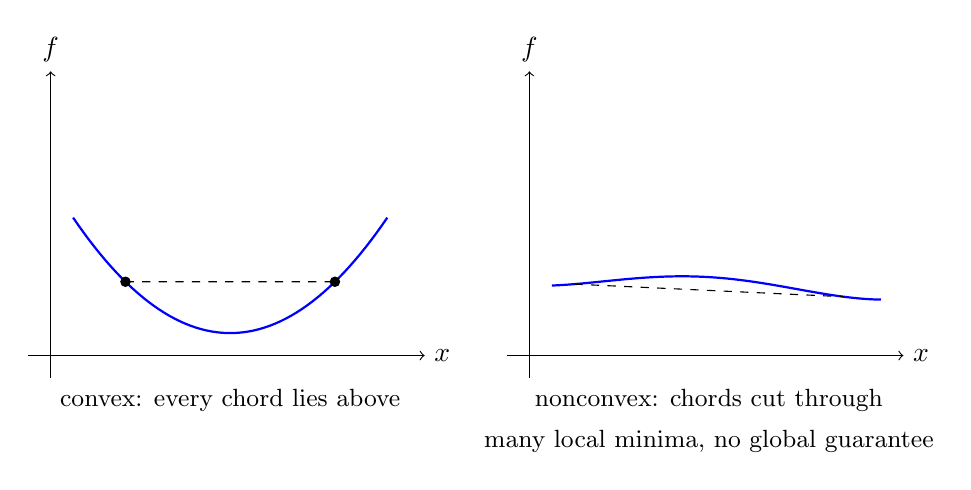
\begin{tikzpicture}[scale=0.95]
% convex bowl
\begin{scope}
\draw[->] (-0.3,0)--(5,0) node[right]{$x$};
\draw[->] (0,-0.3)--(0,3.8) node[above]{$f$};
\draw[thick,blue,domain=0.3:4.5,samples=60] plot (\x,{0.35*(\x-2.4)^2+0.3});
\draw[dashed] (1.0,{0.35*(1.0-2.4)^2+0.3}) -- (3.8,{0.35*(3.8-2.4)^2+0.3});
\fill (1.0,{0.35*(1.0-2.4)^2+0.3}) circle (2pt);
\fill (3.8,{0.35*(3.8-2.4)^2+0.3}) circle (2pt);
\node at (2.4,-0.6) {\small convex: every chord lies above};
\end{scope}
% nonconvex
\begin{scope}[xshift=6.4cm]
\draw[->] (-0.3,0)--(5,0) node[right]{$x$};
\draw[->] (0,-0.3)--(0,3.8) node[above]{$f$};
\draw[thick,blue,domain=0.3:4.7,samples=80] plot (\x,{0.55*sin(200*(\x-0.3)/4.4)+0.09*(\x-2.5)^2+0.5});
\draw[dashed] (0.6,{0.55*sin(200*(0.3)/4.4)+0.09*(0.6-2.5)^2+0.5}) -- (4.2,{0.55*sin(200*(3.9)/4.4)+0.09*(4.2-2.5)^2+0.5});
\node at (2.4,-0.6) {\small nonconvex: chords cut through};
\node at (2.4,-1.15) {\small many local minima, no global guarantee};
\end{scope}
\end{tikzpicture}
